\begin{figure}[tbp] 
  \centering
  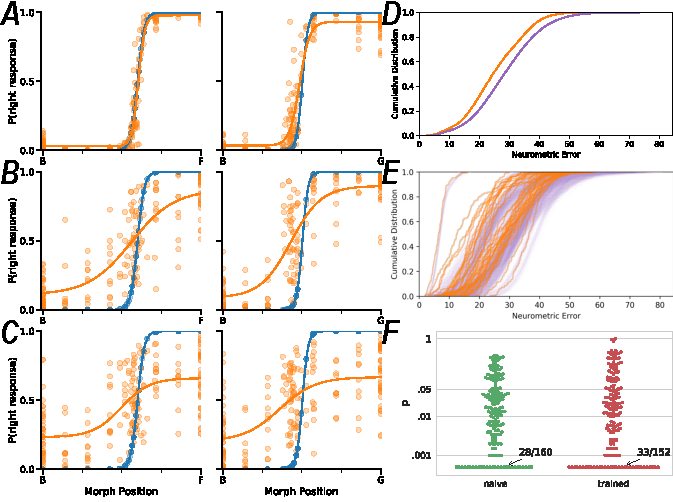
\includegraphics[width=114mm]{figures/fig08_neurometric.pdf}
  \caption[Predicting psychometric curves from neural population activity]
{
(A-C)   Predictions of behavioral psychometric curves for two morph dimensions, left: B to F, right:B to G, for the same behavioral bird, using three different recorded neural populations of differing quality. (A) shows an excellent fit, (B) shows a good fit, and (C) shows a fair fit for these two morph dimensions. Plotted in blue is the behavioral target, and plotted in orange are the held out predictions from a logistic regression trained on the other $15/16$ morph dimensions. The orange dots are the predicted probability of each stimuli presentation and the orange line is a 4 parameter logistic curve fit using \MSE to the probabilities. Some populations (A) do a lot better job at predicting the psychometric curves than others (C).
(D) Cumulative Distribution of the \MSE for neural predictions of the psychometric functions in orange and the cumulative distribution of the \MSE for neural predictions of shuffled psychometric functions in purple. This is the complete cumulative distribution for the \MSE for each of the 16 dimensions, for predictions against the psychometric curves of each behavioral bird (8), for all recorded neural populations (39).
(E) Same as (D) except plotted individually for each neural population in orange, and individually for each of 64 shuffles in purple.
(F) Shuffling each population against the behavioral curves 2048 times and comparing the \KS metric between the distributions allows us to estimate the p values for each neural population. Overall we find most population fits to perform better than would be expected by chance. Furthermore, if we split the recorded populations depending on whether they were from birds trained on this task or naive (never having heard the stimuli before) we find no difference in the distribution of p values. That is to say that a \KS test between the distribution of p values obtained for trained birds against the distribution of p values obtained for naive birds fails to reject the null hypothesis with a p value of $p=0.565$.
\index{neurometric}}
  \label{fig:neurometric}
\end{figure}